\section{Monitorización de base de datos mediante Auditoría} 

\subsection{Introducción}
¿Qué es la Auditoría de BD. Es el proceso que permite medir, asegurar, demostrar, monitorear y registrar los accesos a lainformación almacenada en las bases de datos incluyendo la capacidad de determinar:

\begin{itemize} \item Quién accede a los datos.
				 \item Cuándo se accedió a los datos.
				  \item Desde qué tipo de dispositivo/aplicación.
				  \item Desde que ubicación en la Red.
				  \item Cuál fue la sentencia SQL ejecutada.
				  \item Cuál fue el efecto del acceso a la base de datos.
				  
				   \end{itemize}

Es uno de los procesos fundamentales para apoyar la responsabilidad delegada a IT por laorganización frente a las regulaciones y su entorno de negocios o actividad.

\begin{flushleft}

\begin{center}
	
	\end{center}
\begin{itemize}
\subsection{Objetivos Generales de la Auditoría de BD}

Disponer de mecanismos que permitan tener trazas de auditoría completas y automáticasrelacionadas con el acceso a las bases de datos incluyendo la capacidad de generar alertas con el objetivo de:

\begin{itemize} \item Mitigar los riesgos asociados con el manejo inadecuado de los datos.
				 \item Apoyar el cumplimiento regulatorio.
				  \item Satisfacer los requerimientos de los auditores.
				  \item Evitar acciones criminales.
				  \item Evitar multas por incumplimiento.
				 				  
				   \end{itemize}



La importancia de la auditoría del entorno de bases de datos radica en que es el punto de partidapara poder realizar la auditoría de las aplicaciones que utiliza esta tecnología.



\subsection{Azure Data Studio}

Cuando se trabaja con una base de datos o cualquier otro tipo de software, hay momentos en que la experiencia se ve reforzada o dificultada por las herramientas que utiliza para interactuar con ella.

PostgreSQL tiene una herramienta de línea de comandos, psql y es bastante potente, pero algunas personas prefieren, con mucho, un editor gráfico. Aunque usualmente se usa la línea de comandos, puede que quieran usar una pantalla visual a veces.


Es por eso por lo que Microsoft presentó Azure Data Studio, un editor de GUI de código abierto que admite Postgres.

Microsoft aprovechó la oportunidad para presentar también una vista previa de la extensión PostgreSQL correspondiente en Visual Studio Code (VS Code). Azure Data Studio y VS Code son de código abierto y extensibles, dos elementos en los que se basa PostgreSQL.

\begin{center}
    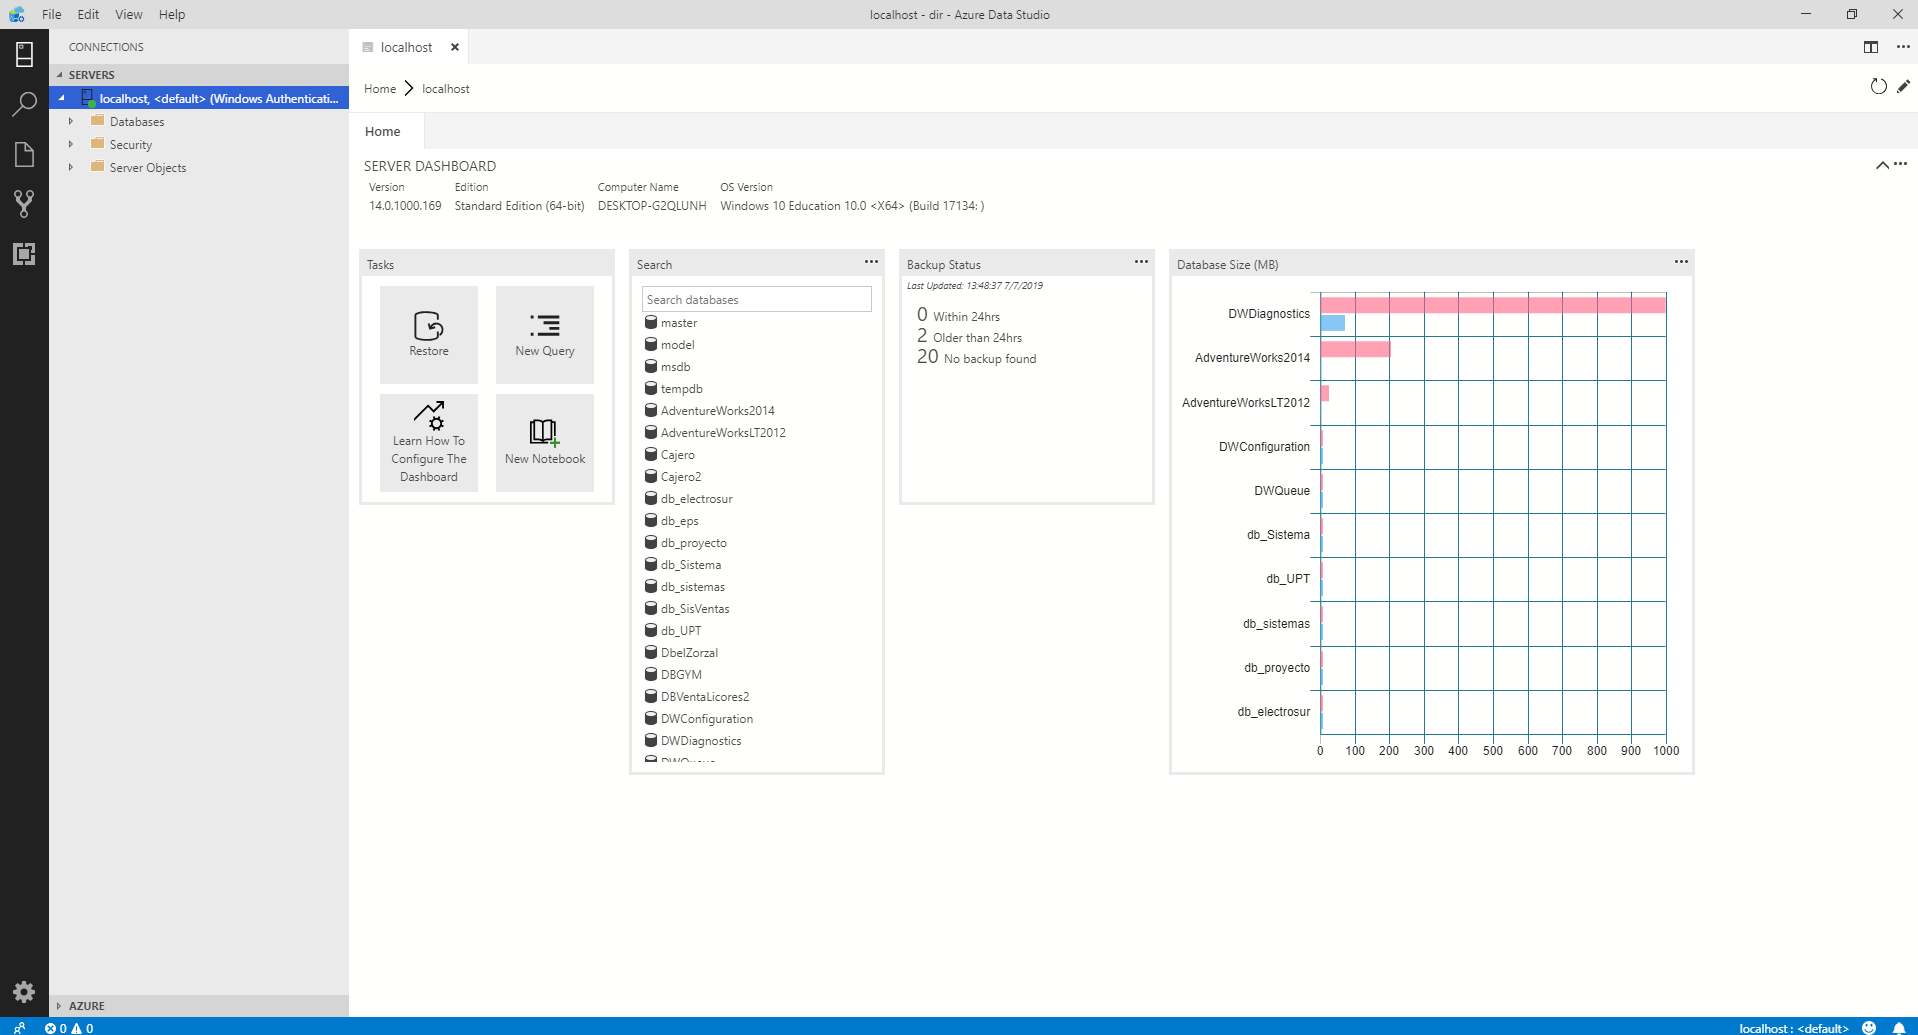
\includegraphics[width=16cm]{./Imagenes/AzureData}
    \end{center}
Azure Data Studio, el editor de código abierto de Microsoft para trabajar con bases de datos SQL, ahora también es compatible con PostgreSQL.

Azure Data Studio está dirigido principalmente a expertos en datos. Por lo tanto, Microsoft también ha desarrollado una extensión de PostgreSQL para Visual Studio Code para aquellos que usan las bases de datos de Postgres como desarrolladores de aplicaciones.

Además, que actualmente se encuentra todavía en una versión de vista previa. Por lo tanto, ambas extensiones de editor podrían contener uno u otro error.

Si su caso de uso principal es la administración de la base de datos, Azure Data Studio puede ser una buena opción.

Pues este permite administrar múltiples conexiones de base de datos, explorar la jerarquía de los objetos de la base de datos, configurar paneles de control y más.
